\chapter{Literatuurstudie}
\label{ch:stand-van-zaken}

% Tip: Begin elk hoofdstuk met een paragraaf inleiding die beschrijft hoe
% dit hoofdstuk past binnen het geheel van de bachelorproef. Geef in het
% bijzonder aan wat de link is met het vorige en volgende hoofdstuk.

% Pas na deze inleidende paragraaf komt de eerste sectiehoofding.


%Dit hoofdstuk bevat je literatuurstudie. De inhoud gaat verder op de inleiding, maar zal het onderwerp van de bachelorproef *diepgaand* uitspitten. De bedoeling is dat de lezer na lezing van dit hoofdstuk helemaal op de hoogte is van de huidige stand van zaken (state-of-the-art) in het onderzoeksdomein. Iemand die niet vertrouwd is met het onderwerp, weet er nu voldoende om de rest van het verhaal te kunnen volgen, zonder dat die er nog andere informatie moet over opzoeken \autocite{Pollefliet2011}.
%
%Je verwijst bij elke bewering die je doet, vakterm die je introduceert, enz. naar je bronnen. In \LaTeX{} kan dat met het commando \texttt{$\backslash${textcite\{\}}} of \texttt{$\backslash${autocite\{\}}}. Als argument van het commando geef je de ``sleutel'' van een ``record'' in een bibliografische databank in het Bib\TeX{}-formaat (een tekstbestand). Als je expliciet naar de auteur verwijst in de zin, gebruik je \texttt{$\backslash${}textcite\{\}}.
%Soms wil je de auteur niet expliciet vernoemen, dan gebruik je \texttt{$\backslash${}autocite\{\}}. In de volgende paragraaf een voorbeeld van elk.

%\textcite{Knuth1998} schreef een van de standaardwerken over sorteer- en zoekalgoritmen. Experten zijn het erover eens dat cloud computing een interessante opportuniteit vormen, zowel voor gebruikers als voor dienstverleners op vlak van informatietechnologie~\autocite{Creeger2009}.



\section{Inleiding}
In dit hoofdstuk zal de lezer ingedompeld worden in de wondere wereld van de virtuele realiteit. Er wordt dieper ingegaan op het technische aspect van VR, de ontwikkelingsomgevingen en soortgelijke applicaties. Men zal ook meer inzicht krijgen in de huidige stand van zaken in de revolutie die virtual reality teweeg brengt. Verder wordt er ook ingegaan op bepaalde revalidatietechnieken die versterkt kunnen worden met VR. Deze literatuurstudie is grotendeels gebaseerd op wetenschappelijke artikels, krantenartikels en educatief beeldmateriaal.

\section{Virtual Reality}

\subsection{Verschil VR - AR - MR}
Vandaag de dag komt men almaar vaker in aanraking met dergelijke termen zoals virtual, augmented en mixed reality. Veel mensen halen deze termen echter nog steeds door elkaar. Ter verduidelijking worden ze daarom hieronder één voor één opgeklaard. Vervolgens zal er ook  gekeken worden welke voordelen bepaalde technologieën met zich kunnen meebrengen die relevant zijn voor het onderzoek. 

\subsubsection{Virtual reality}
Bij het toepassen van deze technologie zal de gebruiker terechtkomen in een virtuele 3D wereld. Hier wordt men dus afgesloten van de echte realiteit, alles wat de gebruiker waarneemt is virtueel. Dankzij bewegingssensoren in de bril en/of controllers worden de bewegingen van de gebruiker weerspiegeld in de virtuele wereld. Enkele bekende VR brillen zijn: de Oculus Rift, HTC Vive en de Samsung Gear VR.

\subsubsection{Augmented reality}
Wanneer men spreekt over augmented reality gaat men de realiteit overladen met virtuele content. Men kan hier dus zeggen dat met behulp van AR de realiteit wordt aangevuld met virtuele, digitale data. Het grote verschil in vergelijking met VR is dat de gebruiker hier wel nog in contact komt met de werkelijkheid terwijl men bij VR helemaal is afgesloten van de realiteit.

\subsubsection{Mixed reality}
Ten slotte kent men ook nog mixed reality, soms ook wel merged reality genoemd. Deze technologie ondervindt invloeden van beide voorgaande technologieën. Hier worden elementen van VR en AR als het ware samengevoegd. Virtuele 3D beelden komen terecht in de echte wereld en men kan hier ook mee interageren zoals in de echte wereld. Dit is meteen ook het grote verschil tussen AR en MR. Augmented reality kan gezien worden als een extra virtuele laag die over de realiteit gelegd wordt terwijl Mixed reality daadwerkelijk de virtuele objecten in de echte wereld zal verwerken.

Onderstaande afbeelding geeft een mooi overzicht van de verschillen tussen de technologieën. In VR zal de eend te zien zijn in een compleet virtuele omgeving, bij AR zal de eend te zien zijn bovenop de reële wereld en tenslotte bij MR zal de eend werkelijk in de omgeving geplaatst worden. MR zal voor de gebruiker dan ook als het meest realistisch waargenomen worden.

\begin{figure}[h]
	\centering
	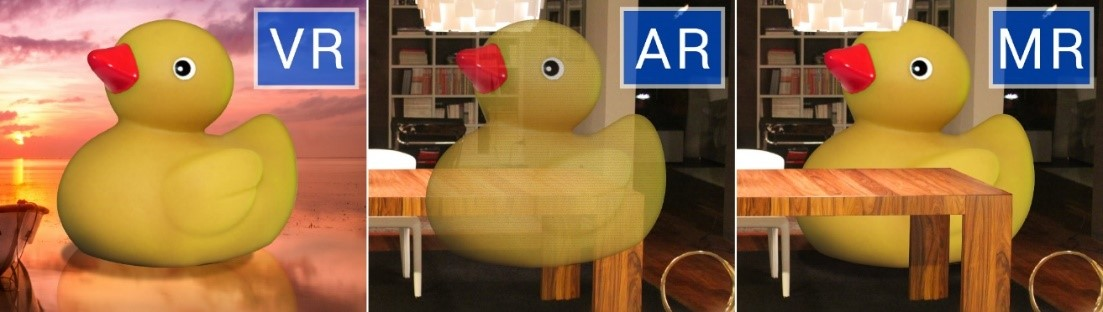
\includegraphics[scale=1.2]{differenceVrArMr.JPG}
	\caption{Visuele voorstelling van verschil tussen VR, AR en MR}
\end{figure}

\subsection{Geschiedenis}

Men zou denken dat virtual reality een relatief jonge technologie is maar niets is minder waar. De fundamenten voor VR werden al veel langer geleden vastgelegd. De beginselen van het begrip rijkt terug naar het jaar 1929. Hier werd de technologie voor de eerste keer gebruikt in een vluchtsimulator ontwikkeld door Edward Link. Deze werd gebruikt om piloten op een veilige manier op te leiden. De zogenaamde ‘Link trainer’ werd ook veel in werking gesteld gedurende de Tweede wereldoorlog.

\begin{figure}[h]
	\centering
	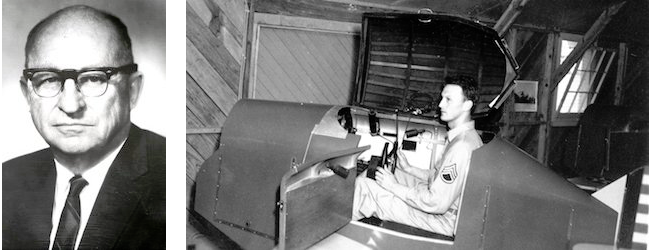
\includegraphics[scale=0.5]{linkTrainer.png}
	\caption{Edward Link en zijn 'link trainer'}
\end{figure}

In de jaren ’50 ontwierp Morton Heilig de Sensorama. Dit was een apparaat gelijkaardig aan een grote kijkdoos die alle zintuigen wist te stimuleren. Wanneer men in de Sensorama plaatsnam maakte het gebruik van geuren, geluiden, beelden en trillingen om de ervaring zo realistisch mogelijk te laten lijken. 

\begin{figure}[h]
	\centering
	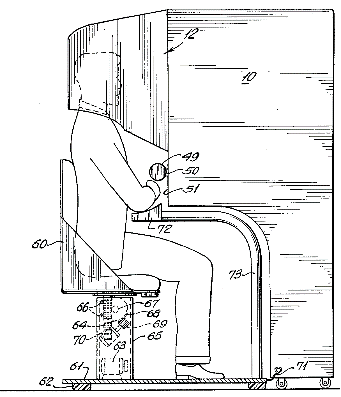
\includegraphics[scale=1]{sensorama.png}
	\caption{De sensorama ontworpen door Morton Heilig}
\end{figure}

In de jaren ’60 kwam Heilig met de eerste Head mounted display, Telesphere mask genoemd. Dit was het eerste voorbeeld van VR zoals we het nu kennen. Deze werkte wel nog niet met motion tracking.
Op deze functionaliteit moest men wachten tot het einde van de jaren ’60 toen ‘The ultimate display’ uit kwam.
Al deze voorgaande uitvindingen sloegen echter niet meteen aan.

Het duurde vervolgens tot in de jaren ’90 voordat de technologie weer wat relevanter werd. Hoewel het voor thuisgebruik nog steeds te duur was konden meer en meer bedrijven het wel al aanschaffen en soms ook beschikbaar stellen voor het publiek. Op die manier kwam het beetje bij beetje al maar meer in de mainstream terecht. Enkele jaren erna sprongen grotere bedrijven zoals onder andere Nintendo mee op de VR trend en brachten VR brillen uit. 

\begin{figure}[h]
    \centering
    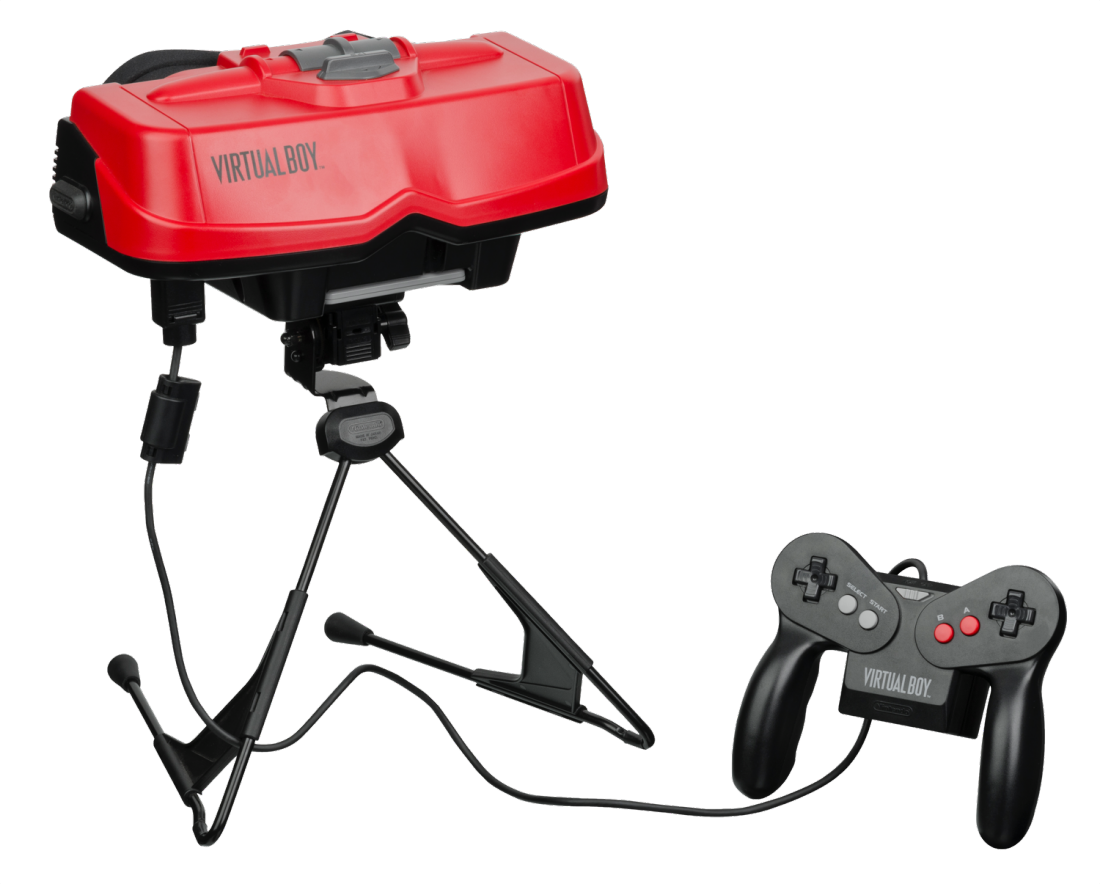
\includegraphics[scale=0.2]{nintendoVr.png}
    \caption{De Virtual boy ontwikkeld door Nintendo}
\end{figure}

\subsection{Bijwerkingen}
\subsubsection{Misselijkheid of 'virtual reality-ziekte'}

De virtual reality ziekte is eigenlijk een vorm van bewegingsziekte of motion sickness. Andere vormen van bewegingsziekte zijn o.a. wagenziekte, zeeziekte, etc. Dit gevoel van misselijkheid is het gevolg van onduidelijke, verschillende signalen die de hersenen binnenkrijgen.

Zo zijn er in het menselijk lichaam drie systemen die ervoor zorgen dat onze positie in de ruimte berekend wordt en we bijvoorbeeld ons evenwicht kunnen houden.
Allereerst gebruiken we onze ogen om onze omgeving waar te nemen. De ogen sturen deze visuele data dan door naar de hersenen en hier wordt deze data dan verwerkt.

Vervolgens hebben we de evenwichtsorganen waar we informatie uithalen. De evenwichtsorganen bevinden zich in het binnenoor van de gebruiker.

\begin{figure}[h]
    \centering
    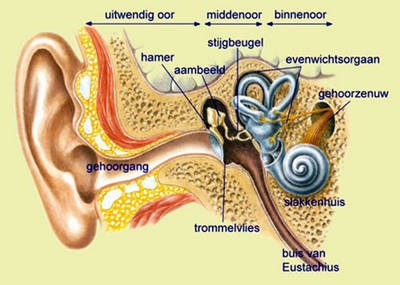
\includegraphics[scale=0.6]{binnenoor.jpg}
    \caption{Het binnenoor met het evenwichtsorgaan}
\end{figure}

Tenslotte beschikken we ook nog over sensoren op de huid en de wervelkolom. Dit vertelt onze hersenen iets over de lichaamshouding van de persoon.

\begin{figure}[h]
    \centering
    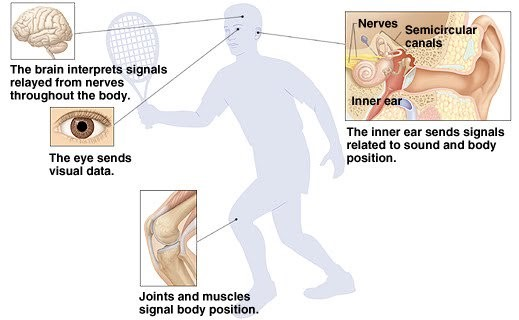
\includegraphics[scale=0.7]{sensoren.jpg}
    \caption{De sensoren van het menselijke lichaam om onze positie in de ruimte te berekenen}
\end{figure}

Wanneer men een VR bril op het hoofd zet kan het soms dan gebeuren dat de hersenen verschillende signalen binnenkrijgen van de ogen en de evenwichtsorganen. De ogen zullen dan bijvoorbeeld denken dat men beweegt maar de evenwichtsorganen dan weer niet. Deze verwarrende signalen zijn dan ook meteen het gevolg van de misselijkheid die men waarneemt. 


De laatste jaren zijn VR ontwikkelaars echter al zeer gevorderd in het verminderen van motion sickness. Dit dankzij grote verbeteringen op vlak van motion tracking en het verhogen van de frame rates van de schermen die men in de headsets verwerkt. Deze factoren zorgen ervoor dat de ogen en de evenwichtsorganen meer en meer op elkaar afgesteld kunnen worden.

\subsubsection{Epileptische aanvallen}
Virtual reality kan ook leiden tot epileptische aanvallen bij bepaalde personen. Er wordt mensen met epilepsie dan ook afgeraden om gebruik te maken van VR headsets. Raadpleeg zeker eerst een arts wanneer u beslist om het toch te doen.

\subsubsection{Hoofdpijn en vermoeide ogen}
Wanneer men te lang naar een computer- of tv-scherm kijkt kan men soms het gevoel krijgen van vermoeide ogen en dat is bij virtual reality ook niet anders. Wat wel verschillend is bij een VR headset is dat men zich in een 3D omgeving bevindt. De ogen zullen zich dus veel frequenter moeten scherpstellen dan wanneer men naar een 2D-scherm kijkt zoals bijvoorbeeld een televisie. De ogen zullen in het algemeen dus wel sneller vermoeid  raken. Vermoeide ogen kunnen soms zorgen voor een minder scherp zicht, hoofdpijn en andere lastige kwaaltjes.Er wordt dan ook door fabricanten aangeraden om regelmatig te pauzeren. De symptomen zijn echter wel slechts tijdelijk, het beste wat je kan doen is rusten. Over de effecten op lange termijn is destijds nog niet veel geweten.



\subsection{Web VR vs Native VR}

\subsection{Verschillende soorten VR headsets}
\subsubsection{Mobile VR}


\subsection{Desktop VR}



\section{Technologieën en ontwikkelingsomgevingen}
\subsection{Game Engines}
\subsubsection{Wat is een game engine?}
Een game engine is werkelijk niets meer dan software die game developers voorziet van de nodige functionaliteiten om op een relatief snelle en efficiënte manier een game te ontwikkelen. In zo een game engine kunnen 2D-, 3D modellen en andere 'assets' ingeladen worden om de gewenste omgeving te creëren. Op die manier zijn er dus oneindig veel mogelijkheden in een game engine. Naast het feit dat men een omgeving kan opbouwen zijn er nog andere elementen waarmee men kan spelen zoals: audio, fysica, netwerkfuncties en interactie met de gebruiker. De wijze  waarop deze elementen met elkaar interageren vormen dan ook de fundamenten van het ontwikkelen van een goede game. Enkele van de meest bekende game engines zijn: Unity en Unreal game engine.
 

bron: https://unity3d.com/what-is-a-game-engine
bron: https://www.gamesradar.com/what-is-a-game-engine-and-what-does-it-do/

\subsubsection{Unity3D}

Unity3D ofwel Unity is een zeer populaire cross-platform game engine ontwikkeld door Unity Technologies.
De eerste versie van Unity kwam in 2005 op de markt, gecreëerd door David Helgason, Joachim Ante en Nicholas Francis. Het was hun doel om een betaalbare game engine te maken die toch geavanceerde functionaliteiten te bieden had voor amateur game developers. Dit was dan ook een van de grootste redenen dat Unity later zo populair werd. Omdat ze geïnspireerd waren door de eenvoudige workflow van Apple programma's was hun eerste versie dus ook enkel toegankelijk voor Mac gebruikers. Hun échte doorbraak kwam echter pas in 2008, gevolgd door het ontstaan van de Apple Iphone en daarbij ook de Apple Appstore. Unity besloot toen om een toegankelijke versie te maken om applicaties voor Iphone's te ontwikkelen. Na hun grote succes op IOS werd het duidelijk dat ze ook een versie voor Windows nodig hadden. Wat Unity vandaag de dag nog steeds zeer populair maakt is het cross-platform element. Momenteel ondersteunt Unity vier categorieën: mobile, web, console en computer. Men kan m.b.v. Unity dus bijna alle publieken bereiken.

bron:https://web.wpi.edu/Pubs/E-project/Available/E-project-030614-143124/unrestricted/Haas\_IQP\_Final.pdf

\subsubsection{Unreal Engine}
Naast Unity hebben we nog een andere veel gebruikte game engine nl. Unreal engine. Deze game engine werd ontwikkeld door Epic Games en werd voor de eerste keer voorgesteld bij de release van de populaire shooter game Unreal in 1998. Deze engine werd vooral gebruikt door de grotere game ontwikkelaars en -studio's. Het was minder populair bij de amateur ontwikkelaar omdat men een abonnement nodig had om toegang te krijgen. Vandaag de dag is Unreal Engine echter volledig gratis.

\subsection{Frameworks}
\subsubsection{Gear VR framework}

\section{Gebruik van VR in gezondheidszorg}
\subsection{Simulatie van behandelingen en operaties}
VR zorgt momenteel al voor grote doorbraken op educatief vlak in de gezondheidszorg. Zo bestaan er al applicaties waar studenten in een virtuele omgeving worden getraind om operaties uit te voeren. Op deze wijze kan een student leren uit zijn/haar fouten zonder cruciale gevolgen. Door operaties al in de praktijk te oefenen stimuleert men het visuele en het fysieke geheugen dat ervoor zorgt dat de handelingen beter onthouden worden. Daarnaast kan virtual reality ook de kosten van training in de gezondheidszorg verlagen. Zo kunnen er meer mensen tegelijk opgeleid worden en moet men niet herhaaldelijk materiaal aankopen voor een bepaalde operatie.

Bron: https://www.td.org/user/content/amirelion/3-great-applications-of-virtual-reality-for-healthcare-training-05-09-18-10-37

In 2017 werkte Oculus samen met CHLA, een kinderziekenhuis in Los Angeles, om een dergelijke training applicatie te ontwikkelen. Studenten worden er blootgesteld aan stressvolle situaties terwijl ze snel beslissingen moeten nemen om een patiënt in leven te houden.

\begin{figure}[h]
    \centering
    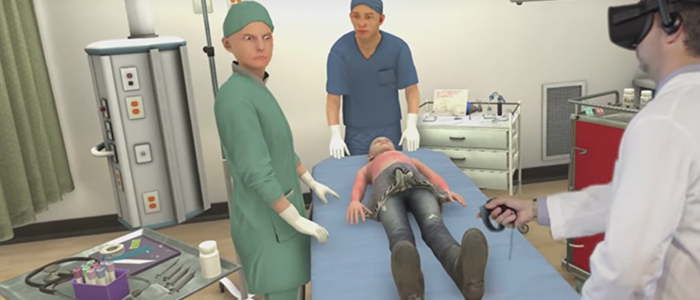
\includegraphics[scale=0.4]{healthApp.jpg}
    \caption{VR simulatie app ontwikkeld door Oculus}
\end{figure}
bron foto: https://theblog.adobe.com/vr-change-healthcare-providers-learn/

Dr. Shafi Ahmed voerde in 2016  als één van de eersten een operatie uit op een gezwel in de darm van een kankerpatiënt terwijl hij deze beelden live uitzond in VR. Op deze manier konden studenten de procedure op de voet volgen alsof ze zelf in de kamer stonden.

\begin{figure}[h]
    \centering
    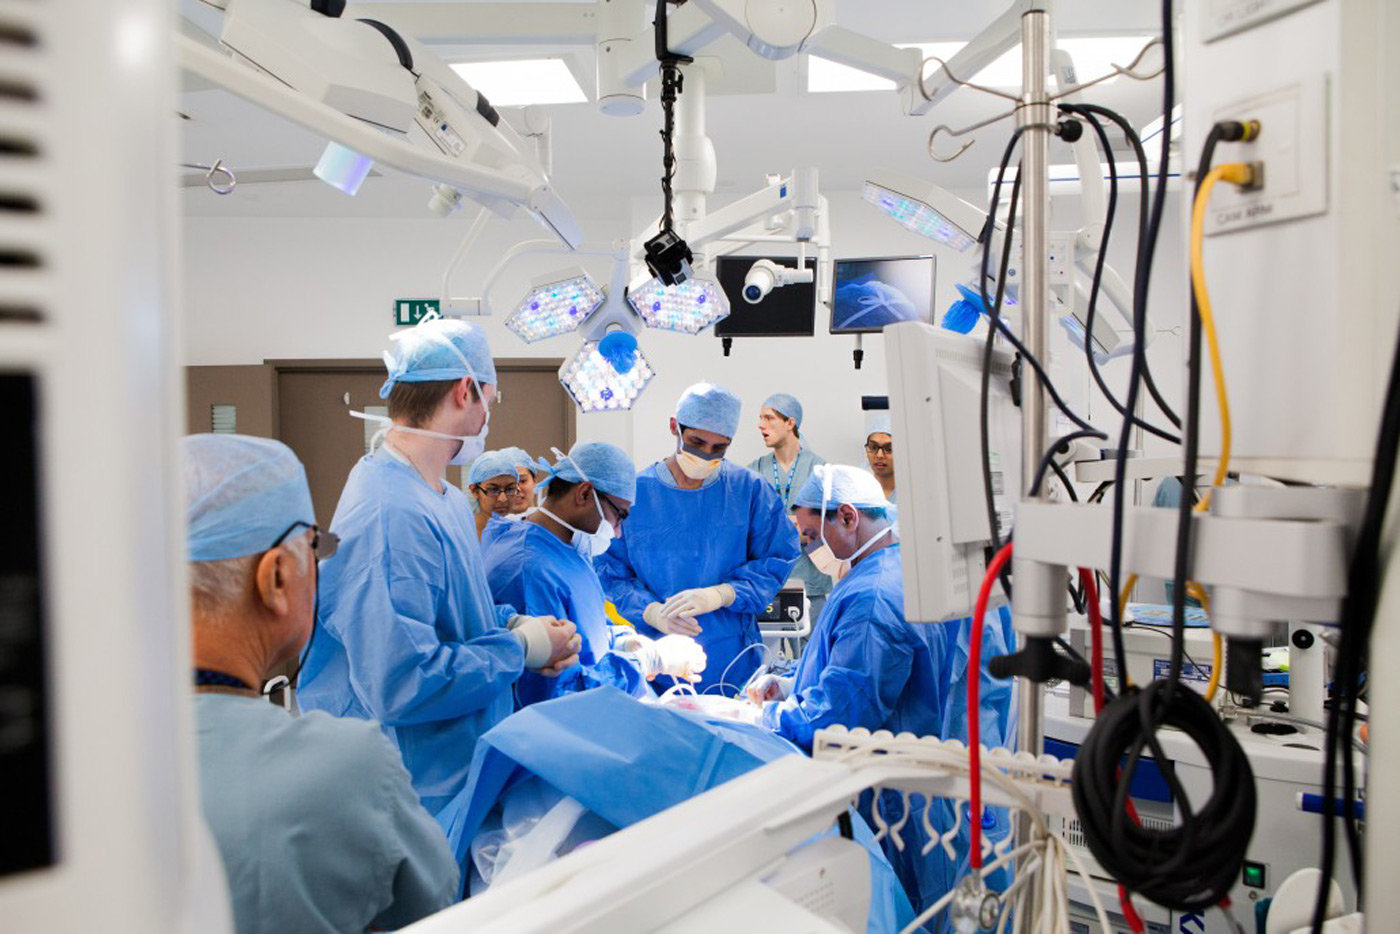
\includegraphics[scale=0.18]{vrOperatie.jpg}
    \caption{Dr. Shafi Ahmed zendt zijn operatie live uit a.d.h.v 360-graden camera's}
\end{figure}

Bron foto: https://www.medicalrealities.com/

Bron: https://www.healthcare.digital/single-post/2017/11/02/The-Benefits-of-Virtual-Reality-in-Healthcare

\subsection{Stress- en angstbeheersing}  
\subsection{Efficiëntere revalidatie na beroerte}  

\section{Focus op revalidatie}
\subsection{Inleiding}
\subsection{Mirror therapy}
\subsection{Distraction therapy}

\section{Soortgelijke applicaties}
\subsection{Mindmotion}
\subsection{VR health}
\subsection{KineQuantum}

